\documentclass{beamer}
\usepackage[utf8]{inputenc}
\usepackage{graphicx}
\usepackage{listings}

\usepackage{xcolor}

\lstdefinestyle{base}{
	language=C++,
	emptylines=1,
	breaklines=true,
	basicstyle=\ttfamily\color{black},
	moredelim=**[is][\bf\color{red}]{@}{@},
}

\usetheme[]{boxes}
\usecolortheme{seagull}

%\usepackage{french}
\title{Modèles et techniques en programmation parallèle hybride et multi-c\oe urs}
\subtitle{Introduction au parall\'elisme multithreads}
\author{Marc Tajchman}\institute{CEA - DEN/DM2S/STMF/LMES}
\date{10/08/2020}

\begin{document}
\begin{frame}
	\titlepage
\end{frame}

\large
\begin{frame}[fragile]
	\section{Parallélisme multi-threads en mémoire partagée}
	\frametitle{Parallélisme multi-threads en mémoire partagée}
	
	Exemple: si \verb|u| et \verb|v| sont des vecteurs de taille \verb|n > 4|, on veut calculer
	\begin{lstlisting}
	v[2] = (u[1] + 2*u[2] + u[3])/4
	v[3] = (u[2] + 2*u[3] + u[4])/4
	\end{lstlisting}
	
	\vfill
	Ces 2 instructions utilisent des composantes de \verb|u| dont certaines sont communes (\verb|u[2]| et \verb|u[3]|) et d'autres sont utilisées par une seule des instructions (\verb|u[1]| et \verb|u[4]|).
	
	\vfill
	\textcolor{blue}{Les composantes de u ne sont pas modifiées par les instructions.
	Les composantes de v sont modifiées (mais chaque instruction calcule une composante différente).}
	
	\vfill
	On remarque que le calcul de v[2] est indépendant de celui de v[3] et donc ces 2 calculs peuvent se faire en même temps par 2 ex\'ecutions différentes qui utilisent les mêmes vecteurs u et v.
		
\end{frame}

\begin{frame}
	\parbox[t][1cm]{10cm}{1. Avant d'exécuter les 2 instructions:}
   \begin{center}
   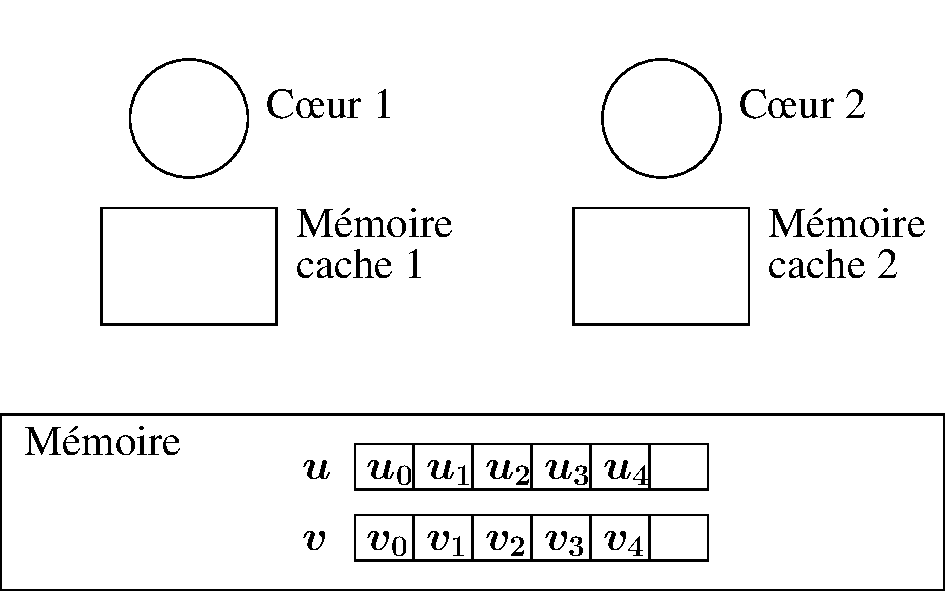
\includegraphics[scale=0.6]{../Images/multithread0}
   \end{center}
\end{frame}

\begin{frame}
	\parbox[t][1cm]{10cm}{2. Les composantes de $u$ sont recopiées dans les mémoires cache:}
   \begin{center}
	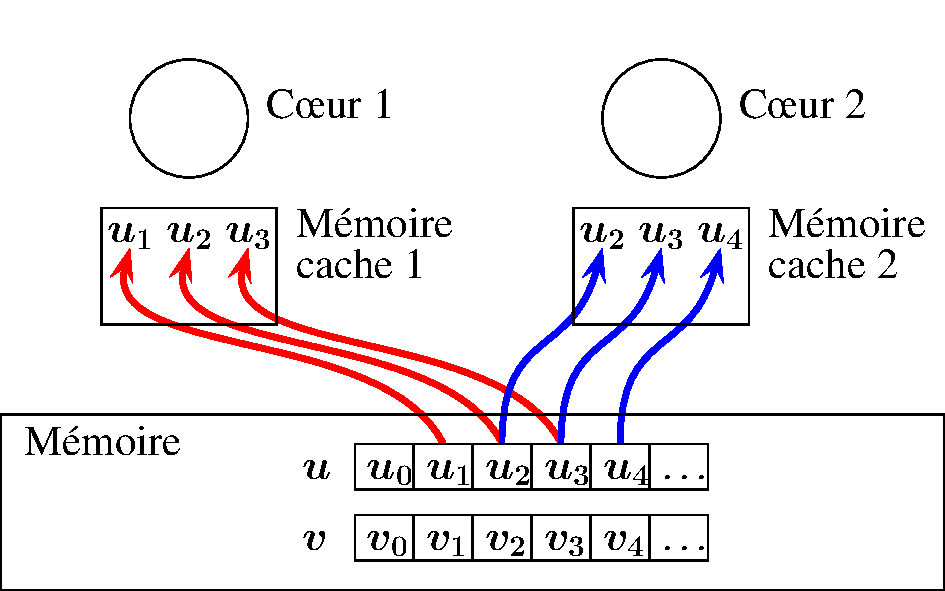
\includegraphics[scale=0.6]{../Images/multithread1}
   \end{center}
\end{frame}

\begin{frame}
	\parbox[t][1cm]{10cm}{3. Les composantes de $u$ sont recopiées dans les mémoires internes des processeurs:}
   \begin{center}
	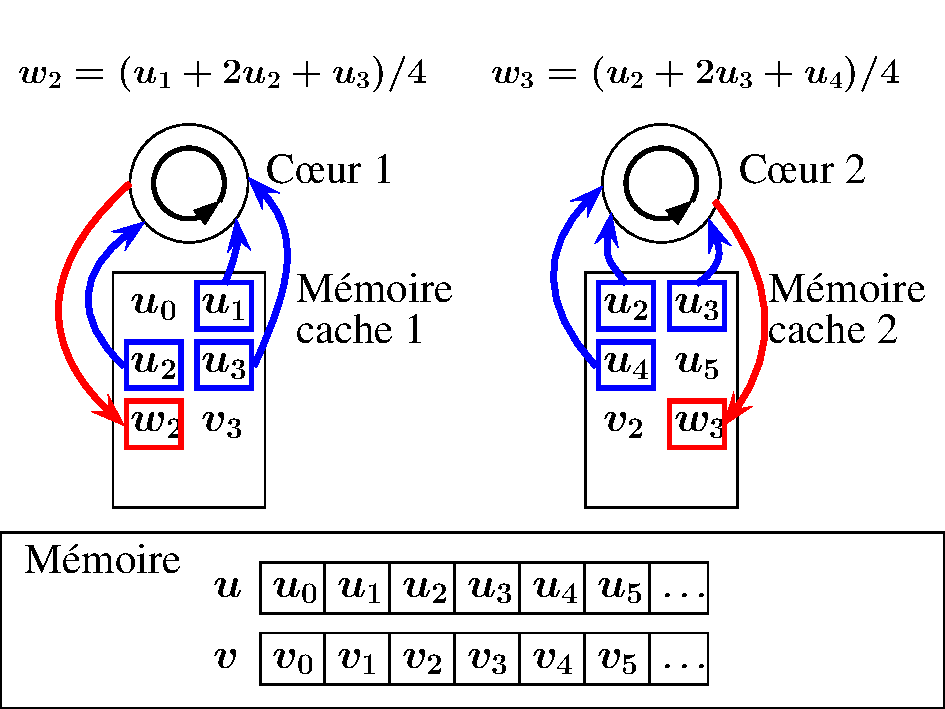
\includegraphics[scale=0.6]{../Images/multithread2}
   \end{center}
\end{frame}

\begin{frame}
	\parbox[t][1cm]{10cm}{4. Le calcul est effectués dans les c\oe urs:
	}
   \begin{center}
	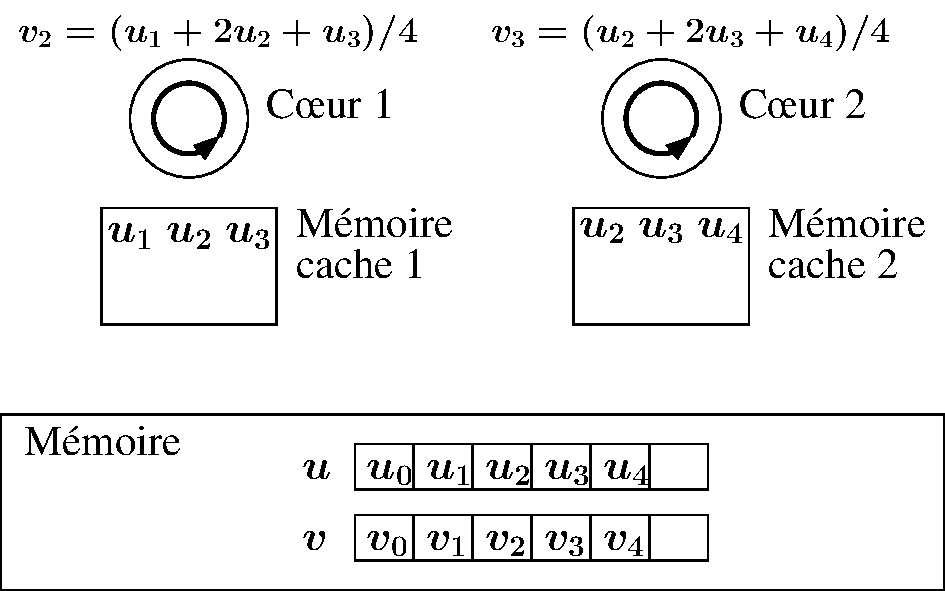
\includegraphics[scale=0.6]{../Images/multithread3}
   \end{center}
\end{frame}

\begin{frame}
	\parbox[t][1cm]{10cm}{5. Le résultat est recopié dans la mémoire cache:}
	\begin{center}
		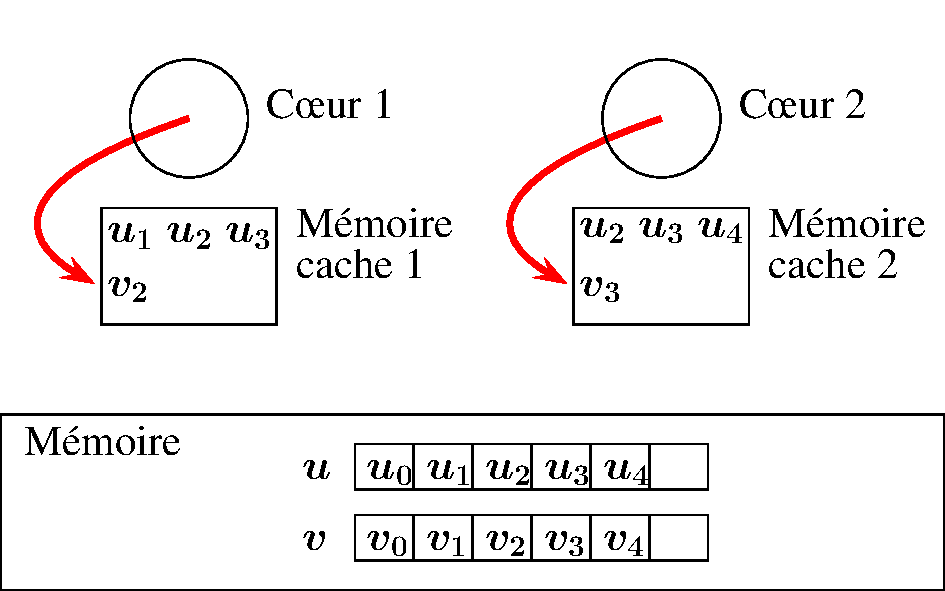
\includegraphics[scale=0.6]{../Images/multithread4}
	\end{center}
\end{frame}

\begin{frame}
	\parbox[t][1cm]{10cm}{6. Le résultat est recopié dans la mémoire principale:}
	\begin{center}
		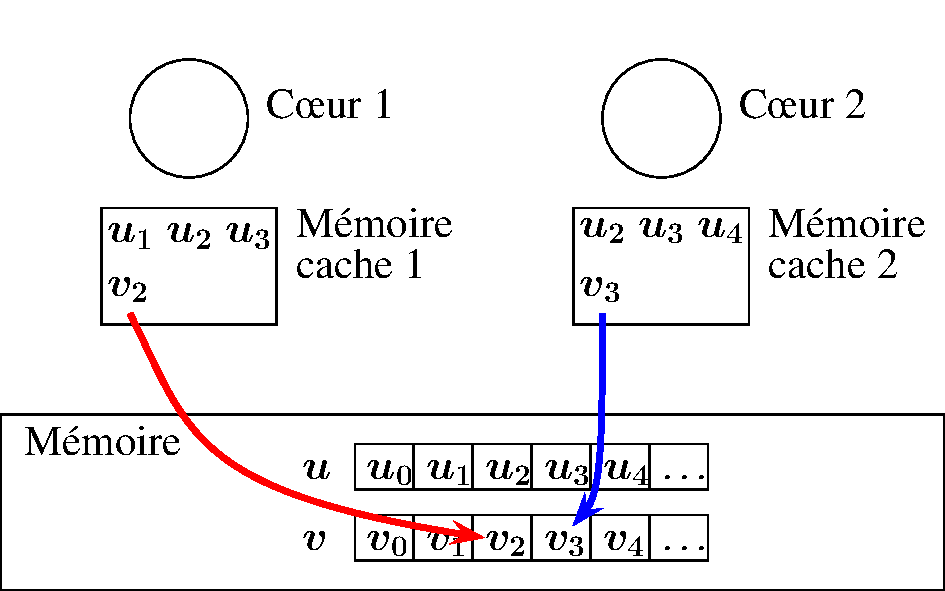
\includegraphics[scale=0.6]{../Images/multithread5}
	\end{center}
\end{frame}

\end{document}